\section{Experiments}
\subsection{Data Sets}
\textbf{Fourclass}. This is a very small data sets we use for test the implementation. It has 862 data points which belong to two classes. Each data point has only two features.

\textbf{vehicle}. The vehicle data set has more data points which is 846 with 18 features. It's combined by 4 classes.

\textbf{MNIST}. This data set is a huge one with 8100000 data points in which are 784 features representing to the pixels. There are 10 classes from 0 to 9. We repeat to choose a very small part randomly from this data set and compute support vectors.

\subsection{Experimental Setup}
Experiments are done on a cluster with Intel Haswell architecture. We use 2 node each with two 12-core 24-thread Xeon E5-2670 processors. All the nodes have 128GB memory and are connected with 1Gbps Ethernet (eth) and Infiniband (ib).

\subsection{Results}
\begin{figure}[htbp]
\centering
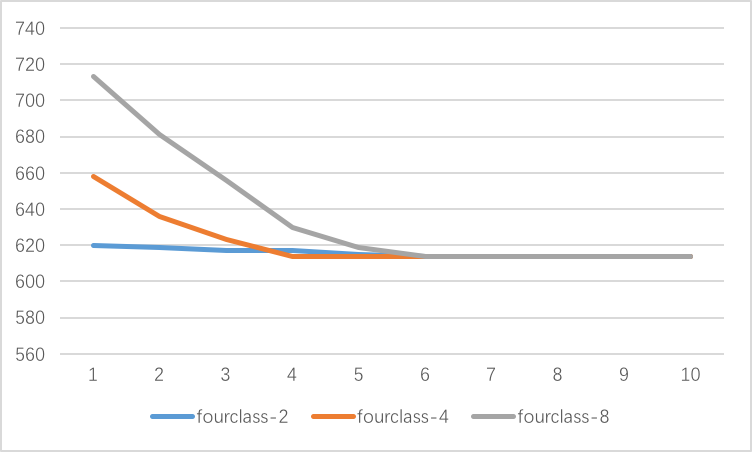
\includegraphics[width=3.0in]{image/SV-fourclass.png}
\caption{The number of support vectors versus the number of iteration on fourclass data set}
\label{SV-fourclass}
\end{figure}

\begin{figure}[htbp]
\centering
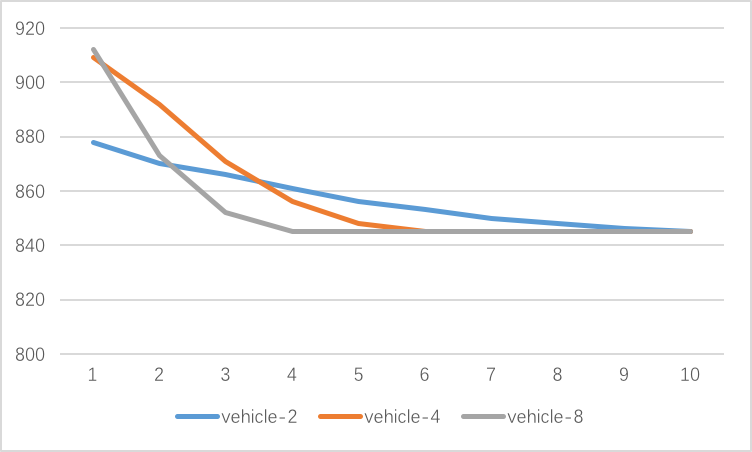
\includegraphics[width=3.0in]{image/SV-vehicle.png}
\caption{The number of support vectors versus the number of iteration on vehicle data set}
\label{SV-vehicle}
\end{figure}

\begin{figure}[htbp]
\centering
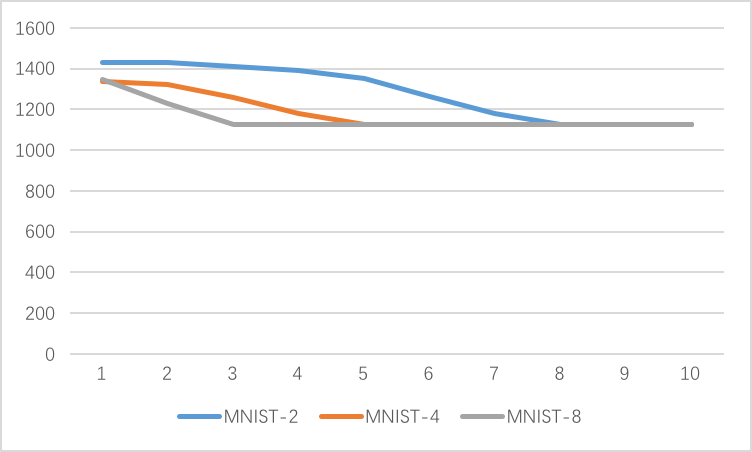
\includegraphics[width=3.0in]{image/SV-MNIST.png}
\caption{The number of support vectors versus the number of iteration on MNIST data set}
\label{SV-MNIST}
\end{figure}

From figure \ref{SV-fourclass} to figure \ref{SV-MNIST} we can see the support vectors' set becomes stable with the increase of the iteration which means that the parallel algorithm works well on training part of data and then merge the support vectors gain by the SVM algorithm. And the more mappers we use, the faster the support vectors' set becomes stable.

While, if we choose to compute by more mappers, the global support vectors at the very beginning is usually larger. That's reasonable because for small data sets, the shape of the clusters can vary from others which means that the support vectors can be very different. So after doing all-reduce, the global vector sets will be larger.

\begin{figure}[htbp]
\centering
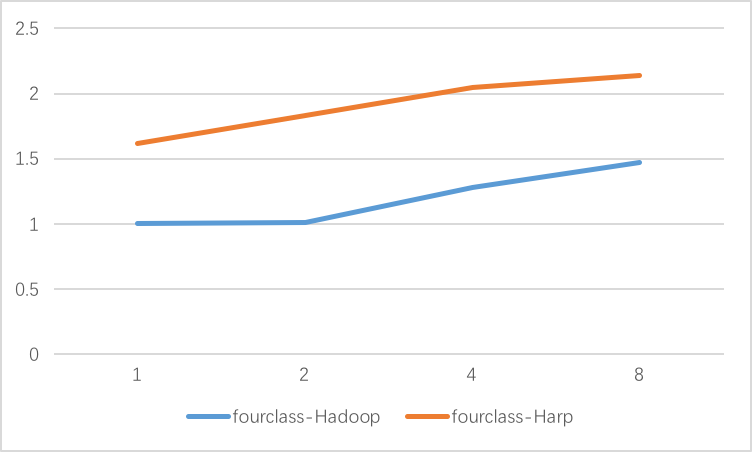
\includegraphics[width=3.0in]{image/speed-fourclass.png}
\caption{Speedup versus the number of mappers on fourclass data set}
\label{speed-fourclass}
\end{figure}

\begin{figure}[htbp]
\centering
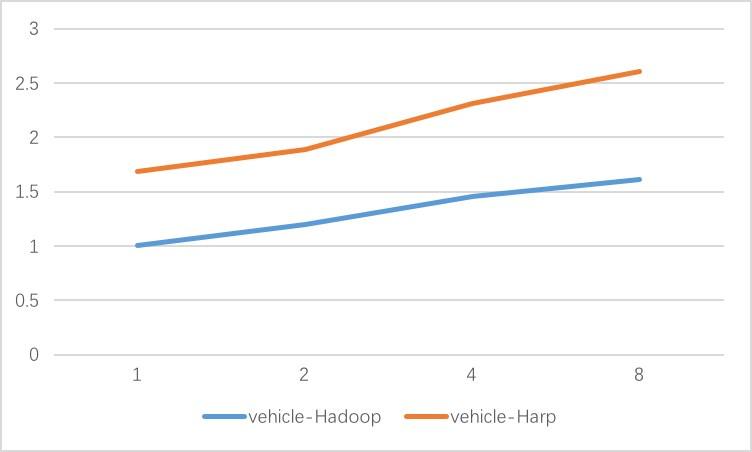
\includegraphics[width=3.0in]{image/speed-vehicle.png}
\caption{Speedup versus the number of iteration on vehicle data set}
\label{speed-vehicle}
\end{figure}

\begin{figure}[htbp]
\centering
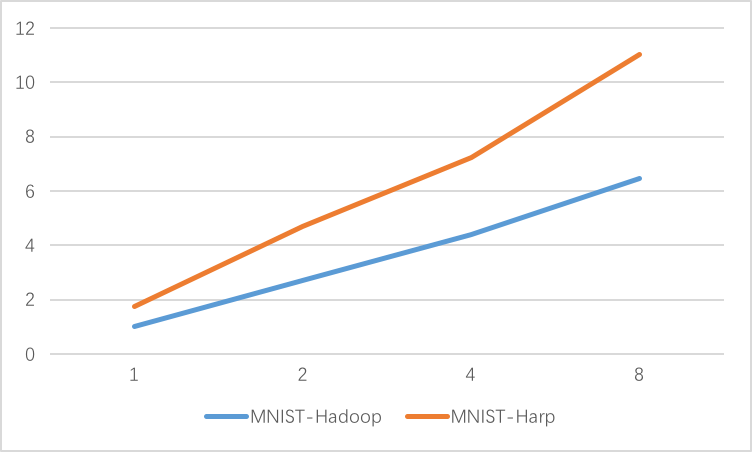
\includegraphics[width=3.0in]{image/speed-MNIST.png}
\caption{Speedup versus the number of iteration on MNIST data set}
\label{speed-MNIST}
\end{figure}

Figure \ref{speed-fourclass} to figure \ref{speed-MNIST} shows that the performance of using Harp is better than only using Hadoop. In the small data sets like fourclass and vehicle, we can see the performance improves at least 40\% and in the MNIST data set, the performance is better 80\% than the Hadoop implementation. The most saving execution time is the I/Os' time. Due to Harp can use all-reduce to synchronize data only through the cache, it will reduce much file reading and writing time which is the indispensable part in Hadoop.


